\documentclass{jsarticle}
\usepackage{amsmath, smssymb, amsfonts}
\usepackage{newtxtext, newtxmath}
\usepackage{latexsym}
\usepackage{mathrsfs}
\usepackage{mathtools}
\usepackage[dvipdfmx]{graphicx, xcolor}
\usepackage{float}
\usepackage{wrapfig}	% must be after float package.
\usepackage{subcaption}
\usepackage{booktabs}
\usepackage{url}
\usepackage{listings, jvlisting, color}

\definecolor{OliveGreen}{rgb}{0.0,0.6,0.0}
\definecolor{Orenge}{rgb}{0.89,0.55,0}
\definecolor{SkyBlue}{rgb}{0.28, 0.28, 0.95}
\lstset{
  language={C++}, % 言語の指定
  basicstyle={\ttfamily},
  identifierstyle={\small},
  commentstyle={\smallitshape},
  keywordstyle={\small\bfseries},
  ndkeywordstyle={\small},
  stringstyle={\small\ttfamily},
  frame={tb},
  breaklines=true,
  columns=[l]{fullflexible},
  numbers=left,
  xrightmargin=0zw,
  xleftmargin=3zw,
  numberstyle={\scriptsize},
  stepnumber=1,
  numbersep=1zw,
  lineskip=-0.5ex,
  keywordstyle={\color{SkyBlue}},     %キーワード(int, ifなど)の書体指定
  commentstyle={\color{OliveGreen}},  %注釈の書体
  stringstyle=\color{Orenge}          %文字列
}


\begin{document}

\title{ゼミ レポート 03}
\author{山田朔也}
\maketitle

\section{本レポートについて}
5月17日に行われたゼミにて出題された課題に対するレポートとなっている。
課題の内容は、llg方程式によって導かれる原子磁気モーメントの反転をシュミレーションすることだ。

\section{問題1}
\subsection{原理}
\subsubsection{磁気モーメント}
磁気モーメントは磁極の対を表す物理量となっている。
このとき、磁極の強さを$q$、磁極の距離を$l$とし、
磁気モーメント自体は$\lvert \vec{M} \rvert = q\vec{l}$と表す。
ここで、距離$l$は磁極の値が負から正の方向に向かうベクトルとするため、
磁気モーメントも負から正への方向へのベクトル量となる。

また、本レポートではCGS単位系を用いるため、$\lvert \vec{M} \rvert$の単位はemuとなる。

\subsubsection{原子磁気モーメント}
原子磁気モーメントは、原子単体が持つ磁気モーメントのことを指す。
また、磁界中に原子磁気モーメントを置くと、原子磁気モーメントは磁界を軸に歳差運動をしつつ
磁界の方向を向いていく。

この運動は Landau-Lifshitz-Gilbert 方程式(LLG方程式)という微分方程式で表される。

\subsubsection{LLG方程式}
LLG方程式は以下の式\ref{01}で表される。
\begin{equation}
	\label{01}
	\dot{\vec{M}} = -\lvert\gamma\rvert(\vec{M}\times\vec{H})+\frac{\alpha}{M}(\vec{M}\times\dot{\vec{M}})
\end{equation}

各変数、$\vec{M}$は原子磁気モーメント、$\vec{H}$は原子磁気モーメントに加わる実効磁界、
$\gamma$は磁気回転比、$\alpha$は損失定数、$M$は原子磁気モーメントの大きさ$(\lvert\vec{M}\rvert)$
となっている。

ここで、原子磁気モーメントを$\vec{M}=M\vec{m}$とおくと、式\ref{01}は
\begin{equation}
	\label{02}
	\dot{\vec{m}} = -\lvert\gamma\rvert\vec{m}\times\vec{H} + \alpha\vec{m}\times\dot{\vec{m}}
\end{equation}
と表せる。また、この式\ref{02}の両辺に$\vec{m}$を掛けて更に整理すると
\begin{equation}
	\vec{m}\times\dot{\vec{m}} = -\lvert\gamma\rvert\vec{m}\times(\vec{m}\times\vec{H}) + \alpha\vec{m}\times(\vec{m}\times\dot{\vec{m}})
\end{equation}
\begin{equation}
	\label{03}
	\Rightarrow\dot{\vec{m}} = \frac{-\lvert\gamma\rvert}{1+\alpha^2}(\vec{m}\times\vec{H} + \alpha(c\vec{m}-\vec{H}))
\end{equation}
となる。ただし、$c=\vec{m}\cdot\vec{H}$とする。

また、この式\ref{03}を3次元空間上で$m_x ,m_y ,m_z$それぞれの式に変えると
\begin{align}
	\dot{m_x} &= \frac{-\lvert\gamma\rvert}{1+\alpha^2}(m_y H_z - m_z H_y + \alpha(cm_x - H_x)) \notag \\
	\dot{m_y} &= \frac{-\lvert\gamma\rvert}{1+\alpha^2}(m_z H_x - m_x H_z + \alpha(cm_y - H_y)) \notag \\
	\dot{m_z} &= \frac{-\lvert\gamma\rvert}{1+\alpha^2}(m_x H_y - m_y H_x + \alpha(cm_z - H_z)) \notag
\end{align}
となる。ただし
\begin{equation}
	\vec{m} = \begin{pmatrix}
				m_x\\ m_y\\ m_z
			  \end{pmatrix}
	,\; \vec{H} = \begin{pmatrix}
					H_x\\ H_y\\ H_z
				\end{pmatrix}
	,\; c = m_xH_x + m_yH_y + m_zH_z
\end{equation}
とする。

\subsubsection{計算モデル}
本問題では、第二回のレポートに示した4次のルンゲクッタ法を用いる。

\subsection{小問1}
\subsubsection{問題内容}
この小問の問題内容は、損失定数を1とし、
外部磁界$(0.001,0,-1)\mathrm{Oe}$を加えた場合の原子磁気モーメントの反転シュミレーションを行い、
結果を2次元および3次元のグラフで示す。但し時間刻みは1ps、磁気回転比は$1.76\times10^7\mathrm{rad/(Oe\cdot s)}$
なお、計算の都度原子磁気モーメントの再規格化を行うこと。
というものとなっている。

\subsubsection{使用したプログラム}
まずは以下に作成したプログラムを記載する。
\begin{lstlisting}[H, caption=4次のルンゲクッタ法で解を得るプログラム, label=list01, language=C++]
	#include <stdio.h>
	#include <stdlib.h>
	#include <stdbool.h>
	#include <string.h>
	#include <math.h>
	#include "solver_RK4.h"
	
	
	
	int main(int argc, char *argv[]) {
		double gamma = 0;
		double alpha = 0.0;
		double dt = 0.0;
		double ku = 0;
		double m[3];
		double H[3];
		double loops = 0;
		int plots = 0;
		init(m, H, &dt, &alpha, &gamma, &ku, &loops, &plots);
	
		int t = 0;
		for (t = 0; t <= loops; t++) {
			RK4(m, H, dt, alpha, gamma, ku);
			if (t % plots == 0) {
				if (strcmp(argv[1], "3") == 0) {
					printout3(m, t);
				} else if (strcmp(argv[1], "2") == 0) {
					printout2(m, t);
				}
			}
		}
		return 0;
	}
	
	// ---------------------------------------
	//	初期設定
	// ---------------------------------------
	int init(double* m, double* H, double* dt, double* alpha, double* gamma, double* ku, double* loops, int* plots) {
		FILE *fp;
		const int n = 256;
		char fname[] = "init.data";
		char line[n];
		char str[16];
		
		fp = fopen(fname, "r");
		if (fp == NULL) {
			printf("init.data not open!\n");
			exit(1);
		}
	
		// 中身の取得
		while(fgets(line, n, fp) != NULL) {
			switch (line[0]){
			case '#':
				break;
			case 'm':
				sscanf(line, "%s %lf %lf %lf", str, &m[0], &m[1], &m[2]);
				break;
			case 'H':
				sscanf(line, "%s %lf %lf %lf", str, &H[0], &H[1], &H[2]);
				break;
			case 'd':
				sscanf(line, "%s %lf", str, dt);
				break;
			case 'a':
				sscanf(line, "%s %lf", str, alpha);
				break;
			case 'g':
				sscanf(line, "%s %lf", str, gamma);
				break;
			case 'l':
				sscanf(line, "%s %lf", str, loops);
				break;
			case 'k':
				sscanf(line, "%s %lf", str, ku);
				break;
			case 'p':
				sscanf(line, "%s %d", str, plots);
				break;
			default:
				break;
			}
		}
	
		/* デバッグ用
		printf("mx: %lf, my: %lf, mz: %lf\n", m[0], m[1], m[2]);
		printf("Hx: %lf, Hy: %lf, Hz: %lf\n", H[0], H[1], H[2]);
		printf("dt: %lf\n", *dt);
		printf("alpha: %lf\n", *alpha);
		printf("gamma: %lf\n", *gamma);
		printf("loops: %lf\n", *loops);
		*/
		return 0;
	}
	
	
	// ---------------------------------------
	//	ルンゲクッタ法
	// ---------------------------------------
	int RK4(double* m, double* H, double dt, double alpha, double gamma, double ku) {
		double k1[3], k2[3], k3[3], k4[4];
		double m0[3];
		int i = 0;
		for (i = 0; i < 3; i++) {
			m0[i] = m[i];
		}
		Euler(m, H, k1, dt, alpha, gamma, ku);
		vadd(m, m0, k1, 0.5);
		Euler(m, H, k2, dt, alpha, gamma, ku);
		vadd(m, m0, k2, 0.5);
		Euler(m, H, k3, dt, alpha, gamma, ku);
		vadd(m, m0, k3, 1.0);
		Euler(m, H, k4, dt, alpha, gamma, ku);
		vadd4(m, m0, k1, k2, k3, k4);
	}
	
	int Euler(double* m, double* H, double* k, double dt, double alpha, double gamma, double ku) {
		double mx = m[0], my = m[1], mz = m[2];
		double Hx, Hy, Hz;
		Heff(m, H, &Hx, &Hy, &Hz, ku);
		llg(k, mx, my, mz, Hx, Hy, Hz, dt, alpha, gamma);
		return 0;
	}
	
	int llg(double* k, double mx, double my, double mz, double Hx, double Hy, double Hz, double dt, double alpha, double gamma) {
		double c = mx*Hx + my*Hy + mz*Hz;
		k[0] = dt * (-fabs(gamma)) * (my*Hz - mz*Hy + alpha*(c*mx - Hx)) / (1 + alpha*alpha);
		k[1] = dt * (-fabs(gamma)) * (mz*Hx - mx*Hz + alpha*(c*my - Hy)) / (1 + alpha*alpha);
		k[2] = dt * (-fabs(gamma)) * (mx*Hy - my*Hx + alpha*(c*mz - Hz)) / (1 + alpha*alpha);
		return 0;
	}
	
	// ---------------------------------------
	//	H に関する計算
	// ---------------------------------------
	int Heff(double* m, double* H, double* Hx, double* Hy, double* Hz, double ku) {
		Hext(H, Hx, Hy, Hz);
		Hanis(m, H, Hx, Hy, Hz, ku);
	}
	
	int Hext(double* H, double* Hx, double* Hy, double* Hz) {
		*Hx = H[0];
		*Hy = H[1];
		*Hz = H[2];
	}
	
	int Hanis(double* m, double* H, double* Hx, double* Hy, double* Hz, double ku) {
		*Hz += 2 * ku * m[3] / sqrt(m[0]*m[0] + m[1]*m[1] + m[2]*m[2]);
	}
	
	// ---------------------------------------
	//	vadd 
	// ---------------------------------------
	int vadd(double* m, double* m0, double* k, double r) {
		int i = 0;
		for(i = 0; i < 3; i++) {
			m[i] = m0[i] + k[i]*r;
		}
	
		double M = sqrt(m[0]*m[0] + m[1]*m[1] + m[2]*m[2]);
		for(i = 0; i < 3; i++) {
			m[i] = m[i]/M;
		}
		return 0;
	}
	
	int vadd4(double* m, double* m0, double* k1, double* k2, double* k3, double* k4) {
		int i = 0;
		for (i = 0; i < 3; i++) {
			m[i] = m0[i] + (k1[i] + 2*k2[i] + 2*k3[i] + k4[i])/6;
		}
	
		double mabs = sqrt(m[0]*m[0] + m[1]*m[1] + m[2]*m[2]);
		for(i = 0; i < 3; i++) {
			m[i] = m[i]/mabs;
		}
		return 0;
	}
	
	
	// ---------------------------------------
	//	出力用関数
	// ---------------------------------------
	int printout2(double* m, int t) {
		int i = 0;
		double ms = (double)t*1.0e-6;
		printf("%lf %.6lf", ms, m[2]);
		printf("\n");
		return 0;
	}
	
	int printout3(double* m, int t) {
		int i = 0;
		for (i = 0; i < 3; i++) {
			printf("%.6lf ", m[i]);
		}
		printf("\n");
		return 0;
	}
\end{lstlisting}
このプログラムの使用方法は、まずは同階層に置いた設定用ファイル「init.data」に必要な初期条件を指定、
そしてプログラムを実行すると、指定した条件からシミュレーションが実行される。
なお、インクルードしている「solver\_RK4.h」はプロトタイプ宣言用に用いている。

結果の出力方法は、標準出力へとなっている。これをテキストファイルに保存して、
gnuplotで表示することで、結果がグラフで示される。

\subsubsection{結果}
次に実際に実行した際の結果を以下の図1に示す。
\begin{figure}[H]
	\centering
	\begin{subfigure}{0.49\columnwidth}
		\centering
		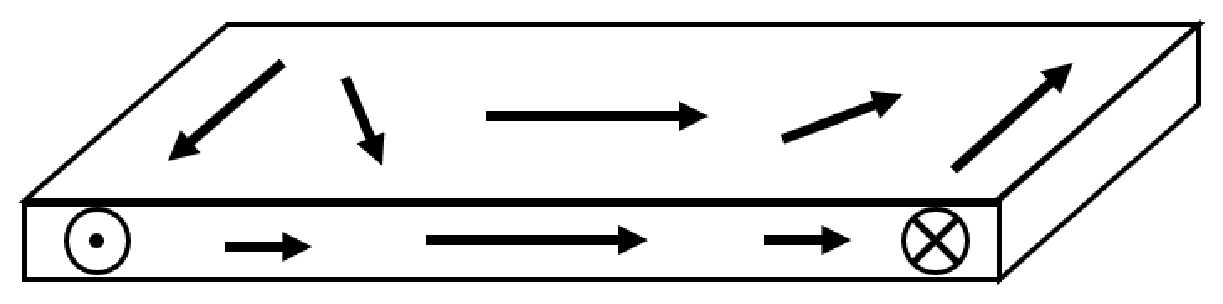
\includegraphics[width=\columnwidth]{pic01.eps}
		\caption{結果を2次元グラフで表した図}
	\end{subfigure}
	\begin{subfigure}{0.49\columnwidth}
		\centering
		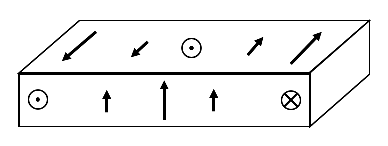
\includegraphics[width=\columnwidth]{pic02.eps}
		\caption{結果を3次元グラフで表した図}
	\end{subfigure}
	\label{fig01}
	\caption{小問1の結果のグラフ}
\end{figure}

これらの図から、原子磁気モーメントは$(0,0,1)$から、外部磁界$(0.001,0,-1)$の方向へと歳差運動をしつつ反転したことが分かる。

\subsection{小問2}
\subsubsection{問題内容}
この小問の問題内容は、損失定数を0.1及び0.01とし、
外部磁界$(0.001,0,-1)\mathrm{Oe}$を加えた場合の原子磁気モーメントの反転シミュレーションを行い、
結果を2次元および3次元のグラフで示す。但し時間刻みは1ps、磁気回転比は$1.76\times10^7\mathrm{rad/(Oe\cdot s)}$
なお、計算の都度原子磁気モーメントの再規格化を行うこと。
というものとなっている。

\subsubsection{結果}
使用したプログラムは小問1と同様のもののため、記載は省略する。
次に実際に実行した際の結果を以下の図\ref{fig02}および図3に示す。
\begin{figure}[H]
	\centering
	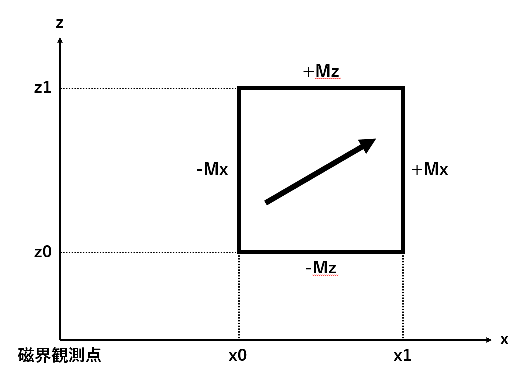
\includegraphics[width=14cm]{pic03.eps}
	\caption{各反転シミュレーションの結果を2次元グラフで表した図}
	\label{fig02}
\end{figure}
\begin{figure}[H]
	\centering
	\begin{subfigure}{0.49\columnwidth}
		\centering
		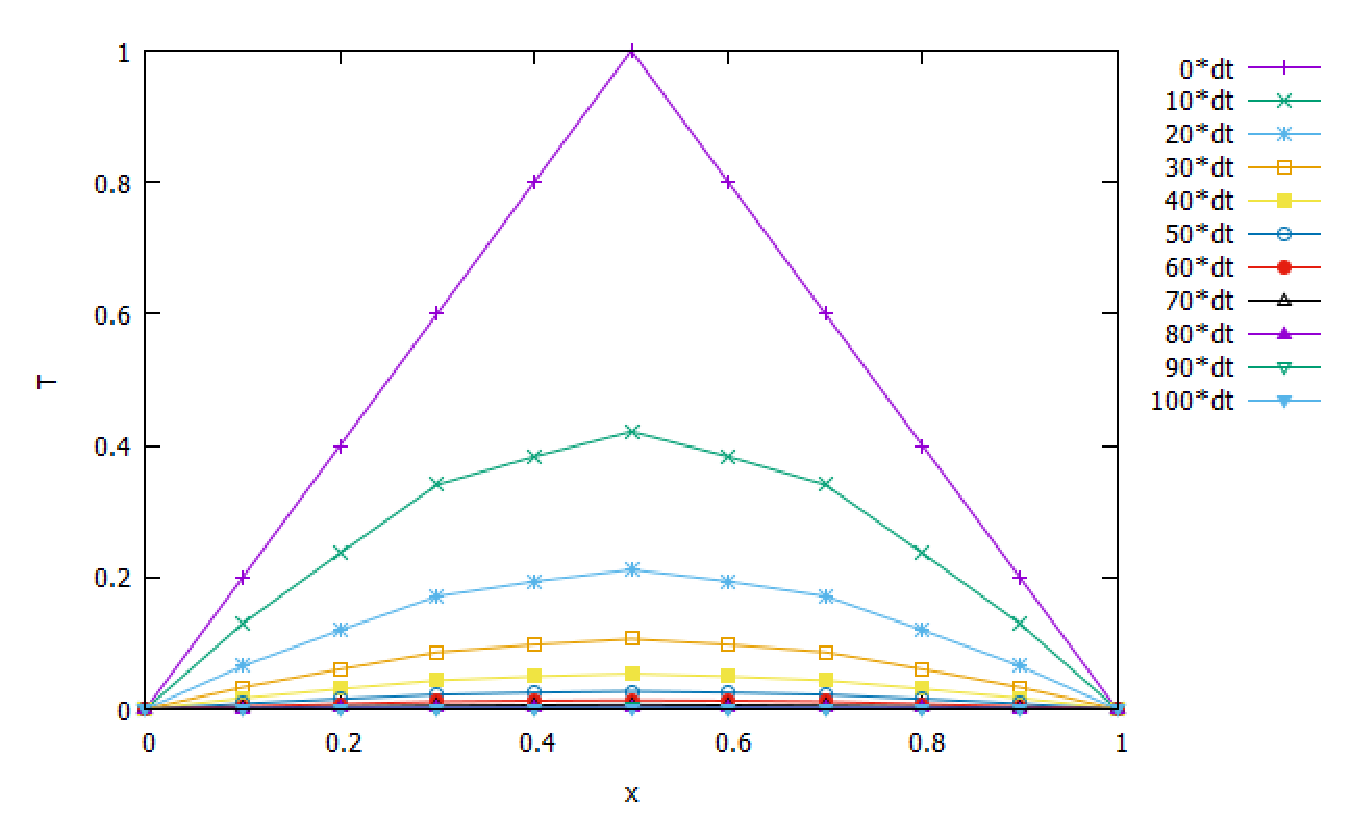
\includegraphics[width=\columnwidth]{pic04.eps}
		\caption{$\alpha=0.1$の時の結果を3次元グラフで表した図}
	\end{subfigure}
	\begin{subfigure}{0.49\columnwidth}
		\centering
		\includegraphics[width=\columnwidth]{pic05.eps}
		\caption{$\alpha=0.01$の時の結果を3次元グラフで表した図}
	\end{subfigure}
	\label{fig03}
	\caption{小問2の結果の3次元グラフ}
\end{figure}

この結果から、$\alpha$の値を小さくすればするほど、原子磁気モーメントが反転するのに多くの時間がかかることが分かる。
ただし、歳差運動自体に影響は殆どなく、原子磁気モーメントが$-1$から$1$の方向へ向かうのに時間がかかっている。
そのため、図3のように反転に時間を掛けた分歳差運動の回数が増えているように見える。

\subsection{小問3}
\subsubsection{問題内容}
この小問の問題内容は、損失定数を0.001から100まで変化させて、反転時間$t_{sw}$の変化を調べる事となっている。

\subsubsection{結果}
使用したプログラムは小問1のものと大きく変わらず、出力する内容を$t_{sw}$に絞ったプログラムとなったため、
記載を省略する。

今回は損失定数が0.001, 0.003, 0.1, 0.3, 1, 3, 10, 30, 100の時の$t_{sw}$を調べ、それをグラフにまとめた。
以下の図\ref{fig04}がそのグラフだ。
\begin{figure}[H]
	\centering
	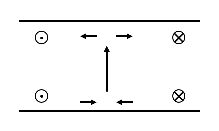
\includegraphics[width=14cm]{pic06.eps}
	\caption{損失定数と反転時間の関係を表すグラフ}
	\label{fig04}
\end{figure}
ここから、損失定数が1の時が最も早く反転し、1から離れれば離れるほど反転時間が長くなる。

\section{問題2}
\subsection{原理}
\subsubsection{一軸磁気異方性}
一軸磁気異方性とは、磁化がある一つの軸方向に向いている時にエネルギーが減少する性質を指す。
このある一つの軸のことを磁化容易軸と呼ぶ。
z軸が磁化容易軸である場合の一軸異方性エネルギーは以下の\ref{04}式で表される。
\begin{equation}
	\varepsilon^K = K_u(1-m_z^2)
	\label{04}
\end{equation}

ここで$K_u$は異方性定数であり、単位は$\mathrm{erg/cm^3}$となる。

このエネルギーを変分することで、エネルギーから磁界への換算が行える。
\begin{equation}
	\vec{H} = -\frac{\delta \varepsilon}{\delta \vec{M}}
\end{equation}
一軸磁気異方性エネルギーの場合、この変換は\ref{05}式で表わされる。
\begin{equation}
	\label{05}
	\vec{H}^K = -\frac{\delta \varepsilon^K}{\delta \vec{M}}
	 = \begin{pmatrix}
		 0\\0\\ \frac{2K_u}{m}m_z
	   \end{pmatrix}
	 = \begin{pmatrix}
		 0\\0\\ H_k m_z
	   \end{pmatrix}
\end{equation}
ここで$H_k$は異方性磁界と呼ばれる。

\subsection{小問1}
\subsubsection{問題内容}
この小問の問題内容は、磁化容易軸がzであり、異方性磁界が$10\mathrm{kOe}$の一軸磁気異方性磁界を考える。
次に、原子磁気モーメントをx-z平面内でz軸から45度傾いた方向$(0, 1/\sqrt{2}, 1/\sqrt{2})$に向け、
その後の磁気モーメントの運動を調べる事となっている。
また、損失定数は0.01、磁気回転比は$1.76\times10^7\mathrm{rad/(Oe\cdot s)}$、時間刻みは1psで計算を行う。

\subsubsection{結果}
計算を行うプログラムは問題1と変わらず、初期条件のみを変更したため省略する。

以下に問題内容に沿った条件でシミュレーションした結果のグラフを、図\ref{fig05}として示す。
\begin{figure}[H]
	\centering
	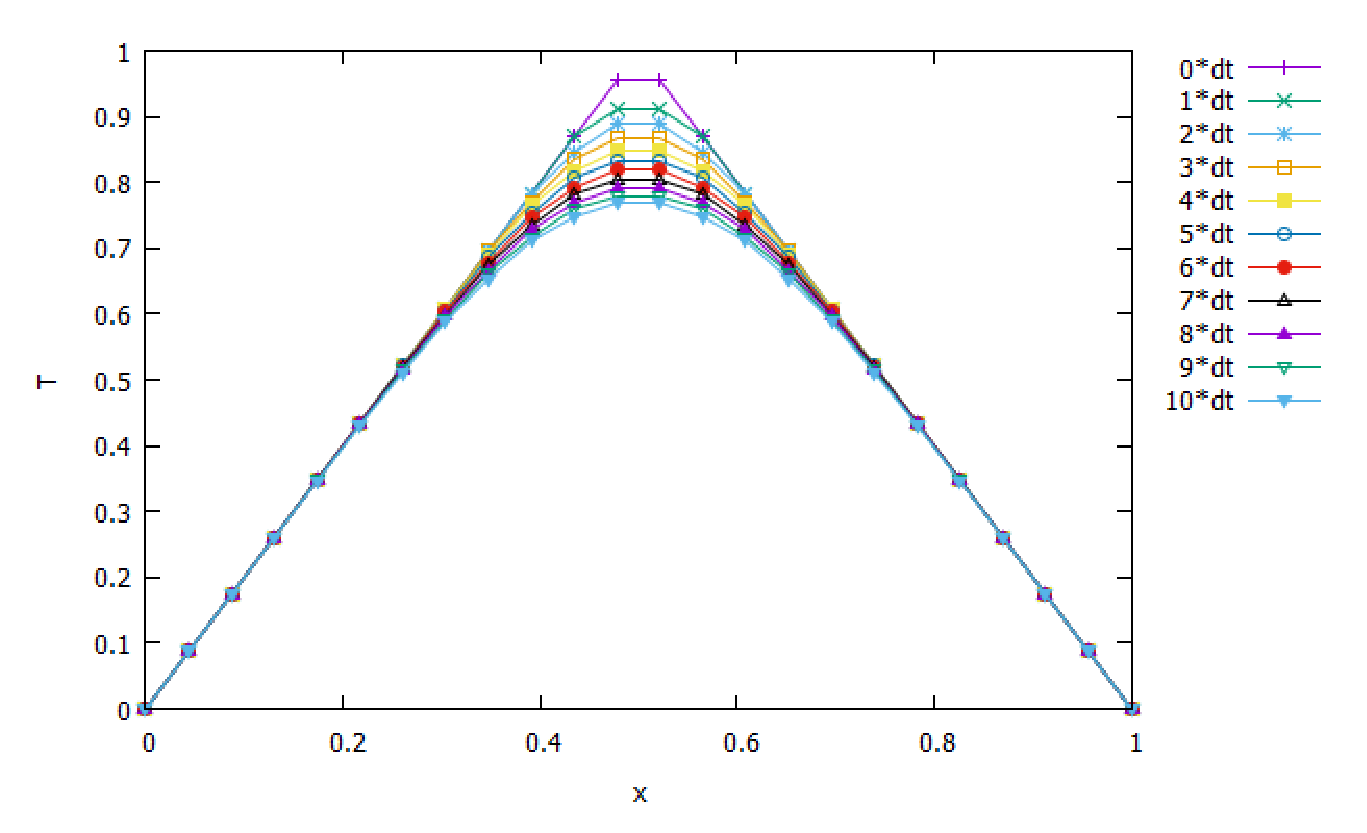
\includegraphics[width=14cm]{pic07.eps}
	\caption{小問1の結果のグラフ}
	\label{fig05}
\end{figure}

このグラフから、初期地点から歳差運動をしつつ一軸磁気異方性磁界の方向へと近づいているのが分かる。

\subsection{小問2}
\subsubsection{問題内容}
この小問の問題内容は、原子磁気モーメントをz軸方向$(0,0,1)$へ向け、
z軸から0.01度傾いた$15\mathrm{kOe}$の外部磁界$(15\mathrm{k}\times\sin(0.01),0,-15\mathrm{k}\times\cos(0.01))$を加え、
反転の様子を調べる。そして、時間刻みを変化させて反転の様子を再度調べる事となっている。

また、上で触れなかった初期条件については小問1を踏襲することとする。

\subsubsection{結果}
計算を行うプログラムは小問1と変わらず、初期条件のみを変更したため省略する。

まず、以下に時間刻みを変化させない状態$dt = 1\mathrm{ps}$でシミュレーションした結果を、
2次元と3次元のグラフで図6として表示する。
\begin{figure}[H]
	\centering
	\begin{subfigure}{0.49\columnwidth}
		\centering
		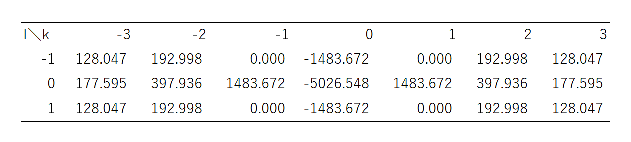
\includegraphics[width=\columnwidth]{pic09.eps}
		\caption{結果を2次元グラフで表した図}
	\end{subfigure}
	\begin{subfigure}{0.49\columnwidth}
		\centering
		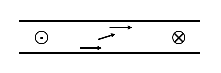
\includegraphics[width=\columnwidth]{pic08.eps}
		\caption{結果を3次元グラフで表した図}
	\end{subfigure}
	\label{fig06}
	\caption{$dt = 1\mathrm{ps}$の結果のグラフ}
\end{figure}

このグラフから、原子磁気モーメントが一軸磁気異方性磁界に逆らい、
外部磁界の方に寄って行っているのが分かる。
これは一軸磁気異方性磁界よりも外部磁界のほうが大きいによりこのような運動をしている。

次に、時間刻みを変化させて反転の様子を調べた結果について。
時間刻みは、まず$1\mathrm{ps}$から$1\mathrm{ps}$ずつ増加させて計算を行っていった。
このとき$8\mathrm{ps}$から原子磁気モーメントは反転をしなくなった。これは更に時間刻みを変化させても反転することはなかった。

そして、時間刻みを$1\mathrm{ps}$から順に、1/10の値を計算していった。しかし、$0.1\mathrm{fs}$まで計算をしたが、変化はなかった。

以下に$1,\;5,\;8,\;0.1\mathrm{ps},\;0.1\mathrm{fs}$の時の反転の様子をまとめたグラフを、図\ref{fig07}として示す。
\begin{figure}[H]
	\centering
	\includegraphics[width=14cm]{pic10.eps}
	\caption{時間刻みを変化させた時の反転の様子}
	\label{fig07}
\end{figure}

この結果から、今回の初期条件においては時間刻みを$8\mathrm{ps}$以上の値に設定すると反転しなくなる。
つまり、計算が破綻することがわかった。
また、時間刻みを小さくしても計算が破綻することはなかった。

\subsection{小問3}
\subsubsection{問題内容}
この小問の問題内容は、外部磁界を変化させて計算を行い、外部磁界と反転時間の関係を調べる。
また、原子磁気モーメントが反転する最小の磁界を求める事となっている。

また、上で触れなかった初期条件については小問2を踏襲することとする。

\subsubsection{結果}
外部磁界を、$1.0\mathrm{kOe}$から$0.1\mathrm{kOe}$ずつ増加させて反転時間を調べていった。
このとき、原子磁気モーメントが反転する最小の磁界は$9.2\mathrm{kOe}$となった。

以下に横軸が外部磁界で、縦軸が反転時間のグラフを、図\ref{fig08}として示す。
\begin{figure}[H]
	\centering
	\includegraphics[width=14cm]{pic11.eps}
	\caption{外部磁界を変化させた時の反転時間の様子}
	\label{fig08}
\end{figure}

また、このグラフから原子磁気モーメント最も早く反転する磁界は$53.4\mathrm{kOe}$だということも分かる。

\section{参考文献}

\begin{itemize}
  \item 配布されたLLGのテキスト
\end{itemize}

\end{document}